\documentclass[letterpaper]{article}
\usepackage[margin=0.5in]{geometry} % Smaller margins for composite diagram
\usepackage[svgnames,dvipsnames]{xcolor}

\usepackage{amsmath}
\usepackage{array}
\usepackage{tabularx}
\usepackage{tikz}
\usetikzlibrary{
    positioning,
    shapes.geometric,
    arrows.meta,
    decorations.pathmorphing,
    calc
}

% --- GLOBAL STYLE DEFINITIONS ---
\tikzset{
    connective_node/.style={
        rectangle, rounded corners=5pt, draw=black!80, fill=black!10,
        inner sep=5pt, thick, align=center
    },
    intro_rule_node/.style={
        rectangle, rounded corners=5pt, draw=black!80, fill=Teal!20,
        inner sep=5pt, thick, align=center
    },
    elim_rule_node/.style={
        rectangle, rounded corners=5pt, draw=black!80, fill=BurntOrange!20,
        inner sep=5pt, thick, align=center
    },
    proposition_node/.style={
        ellipse, draw=black!80, fill=Violet!15,
        inner sep=3pt, align=center
    },
    proof_node/.style={
        ellipse, draw=black!80, fill=Green!15,
        inner sep=3pt, align=center
    },
    input_port/.style={
        circle, draw=blue!70!black, fill=blue!20,
        inner sep=2pt, minimum size=8pt
    },
    output_port/.style={
        circle, draw=ForestGreen!80!black, fill=ForestGreen!20,
        inner sep=2pt, minimum size=8pt
    },
    input_arrow/.style={-Stealth, solid, thick, draw=blue!70!black},
    output_arrow/.style={double, double distance=1.5pt, -Stealth, solid, thick, draw=ForestGreen!80!black},
    proves_arrow/.style={-Stealth, decorate, decoration={snake, segment length=6pt, amplitude=1pt}, thick, draw=orange!90!black},
    composition_arrow/.style={-Stealth, solid, very thick, draw=purple!70!black}
}

% --- Measure width for main theorem box ---
\newlength{\theoremwidth}
\settowidth{\theoremwidth}{$\forall P Q : \text{Prop}, P \land Q \to Q \land P$}
\addtolength{\theoremwidth}{2em}

\begin{document}

\begin{figure}[h!]
\centering
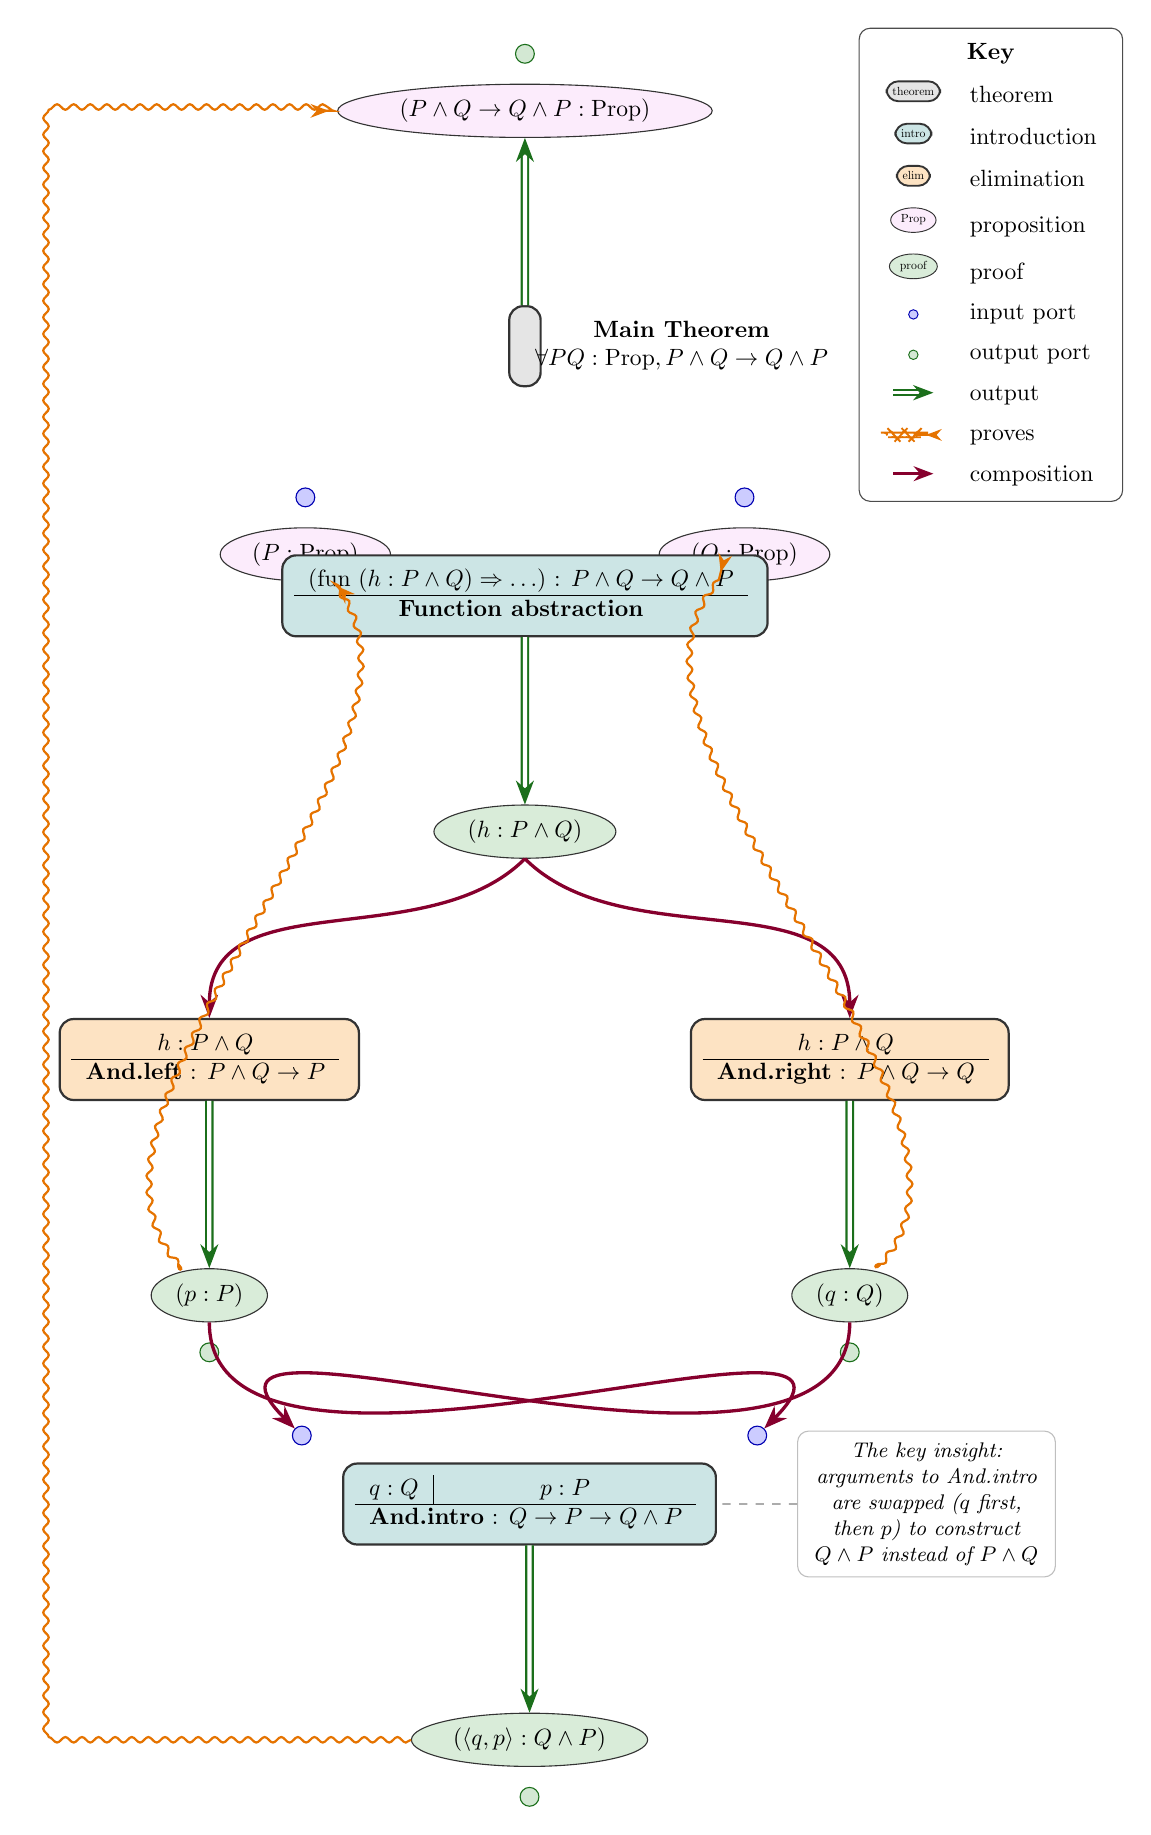
\begin{tikzpicture}[node distance=2.5cm and 2cm, scale=0.85, every node/.style={transform shape}]

% --- TYPE PARAMETERS (SHARED) ---
\node[proposition_node] (P_param) {$(P : \text{Prop})$};
\node[proposition_node] (Q_param) [right=4cm of P_param] {$(Q : \text{Prop})$};

% Input ports for type parameters
\node[input_port] (P_in_port) [above=0.3cm of P_param] {};
\node[input_port] (Q_in_port) [above=0.3cm of Q_param] {};

% --- MAIN THEOREM BOX ---
\node[connective_node, above=2.5cm of $(P_param)!.5!(Q_param)$] (main_theorem) {
    \begin{tabularx}{\theoremwidth}{c}
        \textbf{Main Theorem} \\
        $\forall P Q : \text{Prop}, P \land Q \to Q \land P$
    \end{tabularx}
};

% The constructed implication type
\node[proposition_node] (PandQ_to_QandP) [above=2.5cm of main_theorem] {$(P \land Q \to Q \land P : \text{Prop})$};

% Output port for final theorem
\node[output_port] (theorem_out_port) [above=0.3cm of PandQ_to_QandP] {};

% --- IMPLICATION INTRODUCTION ---
\node[intro_rule_node, below=2.5cm of main_theorem] (implies_intro) {
    \begin{tabular}{c}
    $(\text{fun } (h : P \land Q) \Rightarrow \ldots)$ : $P \land Q \to Q \land P$ \\ \hline
    \textbf{Function abstraction}
    \end{tabular}
};

% The assumption we're abstracting over
\node[proof_node] (h_assumption) [below=2.5cm of implies_intro] {$(h : P \land Q)$};

% --- AND ELIMINATION COMPONENTS ---
\node[elim_rule_node, below left=2.5cm and 1.5cm of h_assumption] (and_left_elim) {
    \begin{tabular}{c}
    $h : P \land Q$ \\ \hline
    \textbf{And.left} : $P \land Q \to P$
    \end{tabular}
};

\node[elim_rule_node, below right=2.5cm and 1.5cm of h_assumption] (and_right_elim) {
    \begin{tabular}{c}
    $h : P \land Q$ \\ \hline
    \textbf{And.right} : $P \land Q \to Q$
    \end{tabular}
};

% Extracted components with ports
\node[proof_node] (p_extracted) [below=2.5cm of and_left_elim] {$(p : P)$};
\node[proof_node] (q_extracted) [below=2.5cm of and_right_elim] {$(q : Q)$};

\node[output_port] (p_out_port) [below=0.3cm of p_extracted] {};
\node[output_port] (q_out_port) [below=0.3cm of q_extracted] {};

% --- AND INTRODUCTION (SWAPPED) ---
\node[intro_rule_node, below=2.5cm of $(p_extracted)!.5!(q_extracted)$] (and_intro_swap) {
    \begin{tabular}{c|c}
    $q : Q$ & $p : P$ \\ \hline
    \multicolumn{2}{c}{\textbf{And.intro} : $Q \to P \to Q \land P$}
    \end{tabular}
};

% Input ports for swapped arguments
\node[input_port] (q_in_port_swap) [above left=0.3cm and 0.5cm of and_intro_swap] {};
\node[input_port] (p_in_port_swap) [above right=0.3cm and 0.5cm of and_intro_swap] {};

% Final result
\node[proof_node] (qp_pair) [below=2.5cm of and_intro_swap] {$(\langle q, p \rangle : Q \land P)$};

% Output port for final result
\node[output_port] (final_out_port) [below=0.3cm of qp_pair] {};

% --- MAIN STRUCTURAL ARROWS ---
\draw[output_arrow] (main_theorem) -> (PandQ_to_QandP);
\draw[output_arrow] (implies_intro) -> (h_assumption);

% --- ELIMINATION FLOW ---
\draw[composition_arrow] (h_assumption.south) to[out=-135, in=90] (and_left_elim.north);
\draw[composition_arrow] (h_assumption.south) to[out=-45, in=90] (and_right_elim.north);

\draw[output_arrow] (and_left_elim) -> (p_extracted);
\draw[output_arrow] (and_right_elim) -> (q_extracted);

% --- INTRODUCTION FLOW (SWAPPED) ---
\draw[composition_arrow] (q_extracted.south) to[out=-90, in=135] (q_in_port_swap);
\draw[composition_arrow] (p_extracted.south) to[out=-90, in=45] (p_in_port_swap);

\draw[output_arrow] (and_intro_swap) -> (qp_pair);

% --- TYPE PROVES ARROWS ---
\draw[proves_arrow, shorten <=3pt, shorten >=3pt] (p_extracted) to[out=135, in=-45, looseness=0.8] (P_param);
\draw[proves_arrow, shorten <=3pt, shorten >=3pt] (q_extracted) to[out=45, in=-135, looseness=0.8] (Q_param);

% Final proves arrow (routed around the diagram)
\coordinate (final_outset) at ($(P_param.west)+(-2.5cm,0)$);
\draw[proves_arrow, shorten >=3pt] (qp_pair.west) -- (final_outset |- qp_pair.west) -- (final_outset |- PandQ_to_QandP.west) -- (PandQ_to_QandP.west);

% --- ANNOTATIONS ---
\node[draw=gray!50, rounded corners, inner sep=5pt, right=1.2cm of and_intro_swap, text width=3.5cm, align=center, font=\small\itshape] (annotation) {
    The key insight: arguments to And.intro are swapped ($q$ first, then $p$) to construct $Q \land P$ instead of $P \land Q$
};

% Connection line from annotation to the swapped intro rule
\draw[dashed, gray] (annotation.west) -> (and_intro_swap.east);

% --- LEGEND ---
\node (legend) [draw=black!70, rounded corners, inner sep=5pt, above right=0.5cm and 0.8cm of Q_param] {
    \begin{tabular}{cl}
    \multicolumn{2}{c}{\textbf{Key}} \\[1.2ex]
    \tikz{\node[connective_node, scale=0.5] {theorem};} & theorem \\[1.2ex]
    \tikz{\node[intro_rule_node, scale=0.5] {intro};} & introduction \\[1.2ex]
    \tikz{\node[elim_rule_node, scale=0.5] {elim};} & elimination \\[1.2ex]
    \tikz{\node[proposition_node, scale=0.5] {Prop};} & proposition \\[1.2ex]
    \tikz{\node[proof_node, scale=0.5] {proof};} & proof \\[1.2ex]
    \tikz{\node[input_port, scale=0.5] {};} & input port \\[1.2ex]
    \tikz{\node[output_port, scale=0.5] {};} & output port \\[1.2ex]
    \tikz{\draw[output_arrow] (0,0.1) -- (0.6,0.1);} & output \\[1.2ex]
    \tikz{\draw[proves_arrow] (0,0.1) -- (0.6,0.1);} & proves \\[1.2ex]
    \tikz{\draw[composition_arrow] (0,0.1) -- (0.6,0.1);} & composition \\
    \end{tabular}
};

\end{tikzpicture}
\caption{Composite proof of the theorem $\forall P Q : \text{Prop}, P \land Q \to Q \land P$ 
using the modular visual algebra. The proof demonstrates systematic composition: (1) Function 
abstraction introduces the implication by assuming $h : P \land Q$, (2) And elimination 
extracts the components $p : P$ and $q : Q$ from the assumption, (3) And introduction with 
swapped arguments constructs $\langle q, p \rangle : Q \land P$. Purple composition arrows 
show the dataflow between modules, while orange proves arrows establish type relationships. 
The input/output port system enables precise connection points between the modular components, 
demonstrating how complex constructive proofs emerge from systematic combination of elementary 
logical operations.}\label{fig:composite_proof_updated}
\end{figure}

\end{document}